\documentclass[11pt]{article}
\usepackage[final]{acl}
\usepackage{times}
\usepackage{latexsym}
\usepackage[T1]{fontenc}
\usepackage[utf8]{inputenc}
\usepackage{microtype}
\usepackage{graphicx}
\usepackage{booktabs}
\usepackage{amsmath}
\usepackage{tabularx}
\usepackage{xurl}
\hypersetup{pdftitle={Reproducing VADER and Testing Sentiment Robustness on New Short Text Data}}
\setlength{\emergencystretch}{1.5em}
\raggedbottom
\renewcommand{\topfraction}{.95}
\renewcommand{\dbltopfraction}{.95}
\renewcommand{\textfraction}{.05}
\renewcommand{\floatpagefraction}{.8}
\setcounter{topnumber}{2}
\setcounter{dbltopnumber}{2}
\setlength{\textfloatsep}{12pt plus 2pt minus 2pt}
\setlength{\dbltextfloatsep}{12pt plus 2pt minus 2pt}
\setlength{\floatsep}{10pt plus 2pt minus 2pt}
\setlength{\dblfloatsep}{10pt plus 2pt minus 2pt}
\captionsetup{skip=5pt}
\graphicspath{{../figures/}}
\title{Reproducing VADER and Testing Sentiment Robustness on New Short Text Data}
\author{COMP8240 Assessment 3 Project Final Report\\Applications of Data Science\\4 November 2026}
\date{}
\begin{document}
\maketitle
\pagestyle{plain}
\thispagestyle{plain}
\begin{abstract}

This project investigates the reproducibility and transfer of VADER, using the provided evaluation materials, an updated sentiment benchmark and controlled short texts. The 23,703 original evaluation texts were evaluated by both an archived and maintained implementation. The archived one brings out the published twittering-like and editorial match to 3 decimal places, but movie and product match is different. It has been found in a classification audit that there is significant sensitivity for conversion of human intensity ratings and for the averaging convention for F1. Archived macro-F1 on the 3600-item Round 1 test set is 0.549 on DynaSent, and 0.523 on the 720-item Round 2 test set. Paired confidence intervals which cross zero indicate that there is no evidence of improvement under maintenance; similar results come from maintained code. New diagnostic corpus 288-text offers a resource for negation, modification, capitals, punctuation and contrast. Its score changes reveal lexical coverage failures, while independent human validation is yet to be completed. Assistive judgement (human reference) evidence is reported separately to an A preserved in the session. Fully replicated and limited transfer experiments were completed, and boundaries on the claims made by the constructed data were clearly identified.

\end{abstract}

Review-draft status. The creation of a corpus and independent human annotation is still underway and the student's public project repository is yet to be checked. No human ratings, consent records, or annotation agreement statistics have been fabricated. The document in the source package contains results of experiments completed and exact remaining dependencies.


\section{Paper description and justification}

\subsection{Research problem}

In very brief texts, it is frequently possible to convey sentiments by the surrounding context and not through the occurrence of positive or negative words. You can turn around an apparent evaluation using negations. Sometimes it is helpful to reinforce a judgement with a capital or an exclamation mark, and sometimes the contrast within a sentence gives the overall evaluation to a different clause of the sentence. A replication must therefore keep these signals and differentiate between number execution and legitimate interpretation by humans.


Pang and Lee (\hyperlink{ref_pang2008opinion}{2008}) put sentiment analysis under the umbrella of computational analysis of opinions and subjectivity. Wilson et al. (\hyperlink{ref_wilson2005contextual}{2005}) separate out from one another a word's prior polarity and contextual polarity. The need to check negation and contrast, in addition to lexical content coverage, as part of the present project motivates this distinction.


With the selected paper, Hutto and Gilbert (\hyperlink{ref_hutto2014vader}{2014}),\footnote{Source paper: \url{https://ojs.aaai.org/index.php/ICWSM/article/view/14550}.} a human-rated sentiment lexicon is used in combination with contextual heuristics. It offers positive, neutral and negative part scores, in addition to compound sentiment scores. The components are output summaries not calibrated probabilities for the 3 classes. In the experiments of this project there is no specific training to perform for classifiers.


Both intensity association and three-class decisions are explored and assessed on social-media-like documents, movie snippets, product snippets and editorials in the source paper. It is reported to be correlated as an excellent tweet (0.881) and overall F1 0.96. These amounts are related to different questions, correlation being association with human intensity, and F1 being dependent on reference classes and decision thresholds and aggregation. Reconstructed houses are dealt with separately in the present project.


\subsection{Why this paper is suitable}

The work has been published in the International AAAI Conference on Web and Social Media, which is a peer-reviewed Conference. ICWSM has been placed in category A \hyperlink{ref_core2023}{(Computing Research and Education Association of Australasia, 2023)} for the historical CORE2023 entry. This ranking is related to the comparative quality in the context; for the practical realisation of the project there is need of executable resources on the basis of which measurable claims can be made that support the project. The author repository provides an implemented version, lexical resources, and the released evaluation data Hutto (\hyperlink{ref_huttoCode}{2026}). Such artefacts are available to allow a direct comparison with published values.


Eliminating the need for model training by CPU allows the project to be realized. Running the system with separate, and stored and maintained, implementations makes comparison with different versions available, without assuming that present code can be run on the 2014 system to produce the same result.


This is a project that follows an independently selected novel-project approach that involves selecting and justifying the VADER paper, author code and original evaluation data. This unit is covered by the overall criteria in this unit and is determined by selection and justification of the project (\hyperlink{ref_courseCriteria2026}{2026}). Transfer benchmark is provided by DynaSent and newly created experimental material is supplied by the constructed corpus.


Three research questions organise the investigation:


1.         How closely does archived code reproduce the published intensity and classification results on the released original corpora?


2.         How well do archived and maintained VADER transfer to the official test splits of a newer three-class benchmark?


3.         Do controlled textual changes produce sentiment changes that agree with independent human judgements?


The first two questions have observed results. The third currently has behavioural diagnostics and an assistant-judge pilot, while its planned independent human reference evaluation remains outstanding.


\section{Original datasets and evaluation}

\subsection{Released data and input format}

The files that are replicated are those held by the author in his/her archive and not corpora reconstructed from existing websites. The released collections include 4,200 text chunks from tweets, 10,605 snippets from movie productions, 3,708 snippets from products and 5,190 snippets from editorials. The collection of social texts is of around 4,000 adapted ones and there are 200 built-in grammatical tests for use in the tweet. The other collections come from movie reviews and product reviews or opinion articles, according to the original paper. Both document level and sentence level intensity annotations are as released in VADER.\footnote{Original released data: \url{https://github.com/cjhutto/vaderSentiment/blob/44fc044cd877310ee8278a0eadf34bcd50d41d06/additional_resources/hutto_ICWSM_2014.tar.gz}.}


The human ground-truth data consists of a tab-separated file containing an item identifier, human intensity ratings and the text. When splitting each line on the first two tabs, the remainder is still kept as text. Table 1 shows a schematic record. IDs remain as strings with any formatting that would get lost when converting to a number. Before the evaluation, each file is authenticated against the expected item count in the file and the recorded SHA-256.


\begin{table}[t]
\centering\small
\setlength{\tabcolsep}{5pt}
\begin{tabularx}{\columnwidth}{@{}lX@{}}
\toprule
Field & Meaning\\
\midrule
id & Released text identifier, retained unchanged\\
human\_mean & Mean sentence intensity supplied in the archive\\
text & Complete input string, including case and punctuation\\
\bottomrule
\end{tabularx}
\caption{Original record format. The parser reads id \textbackslash{}t human\_mean \textbackslash{}t text. Third-Party IDS Separate -- Separate export of numeric predictions and IDs from those of the third-party source texts.}
\label{tab:user1}
\end{table}

The ID is 1, mean intensity 2.726315789, text starts with ``Somehow I was blessed with''. This prefix is an example of the text field, whereas full input could be accessed from the checksummed archive. The complete original string is retained by the parser.


The original paper refers to 20 human raters, whom were screened. This should not be confused with the word-rating procedure that was conducted to build the lexicon. Released mean ratings will not repeat the original annotation study or re-determine the inter-rater reliability for the original annotation study. The project doesn't replicate all the comparison systems from the paper either. It is replicated to the VADER result in each collection released.


\subsection{Scores and metrics}

The adjusted valence sum $v$ is mapped into a bounded range to give the compound score.


\begin{equation}c=\frac{v}{\sqrt{v^2+15}}.\end{equation}

Classification uses the documented inclusive thresholds: c\ensuremath{\geq}0.05 is positive, c\ensuremath{\leq}-0.05 is negative, and values between them are neutral. These settings stay unchanged during the new-data evaluation.


Each compound prediction is correlated with the mean value calculated from the humans released. A positive linear rescaling of the human ratings leaves this correlation unchanged. Therefore, it is possible to break out all human means by 4 to switch the class labels without altering the correlation outcome. This separation is in the middle of the protocol audit.


The true-positive, false-positive and false-negative numbers are used for precision and recall per class $k$. The main score is for three classes.


\begin{equation}F_{1,\mathrm{macro}}=\frac{1}{3}\sum_{k=1}^{3}\frac{2TP_k}{2TP_k+FP_k+FN_k}.\end{equation}

You will be given zero points if you do not use any of these three classes.If undefined classes are not used, all three will be counted off. Macro-F1 is accompanied with the accuracy, per-class precision/recall/F1 and confusion matrices. Weighted F1 instead gives more weight to the class scores depending on the reference class for that class, and can mask low performance rates of the minority class \hyperlink{ref_sklearnMetrics}{(scikit-learn developers, 2026)}. Until the overall F1 is aggregated, the published overall F1 is kept under the same name.


\section{Replication of original work}

\subsection{Environment and implementation control}

The other tests were performed with the fresh experiments in a Linux environment with Python 3.12.14 without a GPU. The numerical environment used NumPy 2.3.5, Pandas 2.2.3, SciPy 1.17.0, scikit-learn 1.8.0 and Matplotlib 3.10.8. This is due to the source revision being 44fc044c and full commit information, resource checksums and execution metadata are kept in the source package.


The implementation to be used is the compatibility port which is included in the turned-in copy of Assessment 2 notebook. Python 2 syntax has been adapted for Python 3 and the archived lexicon has been decoded with Latin-1. It is integrity checked via source checksum prior to loading. The port or the sentiment rules were not adapted to enhance the degree of agreement with the paper. A file system could not be found at the clone destination.


All 23,703 original items were scored by both implementations. The scripts export per-item compound scores, corpus summaries and per-corpus metadata records. The last repository must be publicly open to the marker(s).\footnote{Student project repository: publication and URL verification pending in this review draft. The accompanying project package contains the readable scripts, dependencies, results, figures and report source needed for the completed experiments.}


\subsection{Use of unit methods and tools}

The included features are scripted Internet retrieval, checksums, Pandas/NumPy data tests, evaluation using SciPy/scikit-learn, Matplotlib graphics figures, and preparation of a document using LaTeX/BibTeX. The focus on reproducible code through accessible code and documented experimental procedures in Pineau et al. (\hyperlink{ref_pineau2021reproducibility}{2021}) is reflected in the functionality of the pinned source revisions and recorded dependencies. The project repository shall include the report, generated data, generation/evaluation scripts and directions, which should be publicised.


\subsection{Observed correlation results}

The fresh run is shown in the Table 2. The reported 0.881 correaltimes of duplicated tweets are due to the archived value of 0.881166. The correlation between the two sessions is 0.491511 or approximately 0.492, which is archived. The movie result is 0.416477 rather than 0.451, an absolute difference of 0.034523. The result of the product is 0.570896 and not 0.565 with an absolute difference of 0.005896. These results are a partial replication.


\begin{table*}[t]
\centering\small
\setlength{\tabcolsep}{5pt}
\begin{tabular}{@{}lrrrrrr@{}}
\toprule
Corpus & Texts & Paper r & Archived r & Maintained r & Paper F1 & \shortstack{Provisional\\macro-F1}\\
\midrule
Tweet-like & 4,200 & 0.881 & 0.881166 & 0.872217 & 0.96 & 0.7467\\
Movie & 10,605 & 0.451 & 0.416477 & 0.427597 & 0.61 & 0.4055\\
Product & 3,708 & 0.565 & 0.570896 & 0.589628 & 0.63 & 0.5131\\
Editorial & 5,190 & 0.492 & 0.491511 & 0.502898 & 0.55 & 0.5206\\
\bottomrule
\end{tabular}
\caption{Original-data replication. The values for published correlation and F1 are copied from the VADER row in Table 4 of the source paper. This metric is for provisional (not published) macro-F1 in addition to the published macro-F1 and is not defined as a relabelling of the published macro-F1.}
\label{tab:user2}
\end{table*}

\begin{figure*}[t]

\centering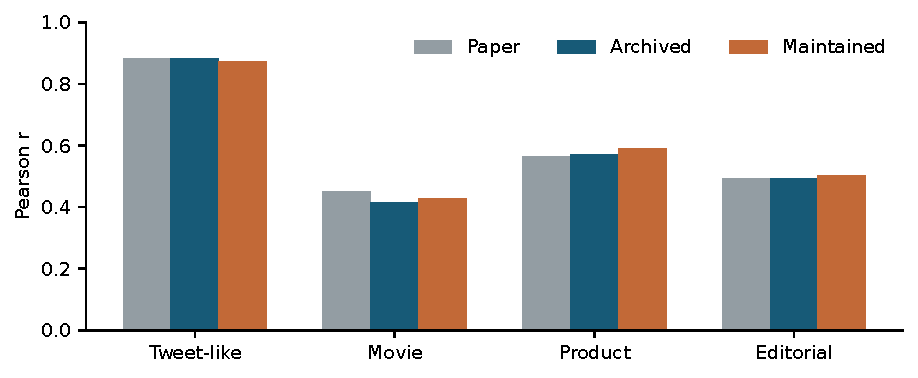
\includegraphics[width=.76\textwidth]{replication_correlations.pdf}

\caption{Reported and reproducible intensity correlations. For everything but Maintained code, there is no guarantee that every collection will get closer to the original published value.}

\label{fig:user1}

\end{figure*}

The maintained implementation produces correlations of 0.872217, 0.427597, 0.589628 and 0.502898 in the same corpus order. It enhances the correlation of the movie with the archived one, but shifts the value of the tweet and product away from their published target values. Thus, it's about the replacement of archived code by "maintained code" and not necessarily about solving the replication problem per se.


The resource comparison reports 7502 lexicon entries in the archive, and another 7506 entries in the maintained resources, with four additions and no removals and two changes in the edited valences in the shared lexicon entries. The implementations also vary in regard to rule processing. This audit does not separate out the causal impact of lexicon change from any changes to the rules. Checksummed inputs and fixed counts minimise the potential for inadvertent changes in local substitutions; they don't guarantee that the same inputs are used during the entire process of creating the artefacts released by a paper.


\subsection{Classification protocol audit}

The policy for the notebook is provisional, meaning it may be revised at any time. Archived tweet-like macro-F1 is 0.746696 under the provisional policy for the notebook. This is well below the overall F1 on the paper of 0.96. The audit assesses pre-defined alternatives to the human mean which are human mean $h$ : the notebook policy ($h/4$), the unscaled released mean ($h$), and the conversion to a nonlinear mapping compatible with a VADER log measurement system ($h/\sqrt{h^2+15}$). The same set of class thresholds are used for both. This is followed by a reporting of macro and weighted aggregation separately.


\begin{table*}[t]
\centering\small
\setlength{\tabcolsep}{5pt}
\begin{tabular}{@{}lrrrr@{}}
\toprule
Corpus & h/4 macro & h macro & h weighted & Paper F1\\
\midrule
Tweet-like & 0.747 & 0.714 & 0.958 & 0.96\\
Movie & 0.405 & 0.397 & 0.585 & 0.61\\
Product & 0.513 & 0.446 & 0.615 & 0.63\\
Editorial & 0.521 & 0.430 & 0.544 & 0.55\\
\bottomrule
\end{tabular}
\caption{Archived classification sensitivity. Different columns differ with respect to reference score scale and F1 averaging, and cannot be compared with respect to the threshold of VADER. The raw-mean/weighted tweet-like value rounds up to 0.96; however, this similarity in numbers is not the same as the original evaluation protocol.}
\label{tab:user3}
\end{table*}

It is particularly telling to see how the level of support these people on the neutral side meant for each side has shifted. In the case of tweet-like text, $h/4$ yields 297 neutral reference items, while the unscaled policy only produces 40. Under the latter policy, weighted F1 is 0.957756 and accuracy is 0.940000; macro-F1 is still only 0.713843. When all of the classes are weighted equally, a high weighted score can, of course, balance much weaker scores.


The raw-mean/weighted result will reproduce the numerical value of the headline F1, however it is not necessary to claim a recovered protocol with this. Normalised threshold and overall metrics are explained in the paper, and these other options give rise to other reference partitions. More importantly, both of the alternate do not "restore" the other collections. The correct result is a clear sensitivity result (as outlined above) not finding an error in the original research.The result should be an explicit sensitivity result, not a statement of 'error in the original paper'. A threshold did not need to be chosen to optimise test scores.


\subsection{Examples from the original data}

For more quality evidence we refer to table 4 which shows the results of the released tweet-like corpus. The quantity of items 4 and 35 is consistent with the derived reference class. Both implementations rate Item 266 with zero for the positive human mean, showing that they do not have to solve the problem in the positive human sense, whereas a rare few do. For item 431, a positive score is given for archived code, while a negative score is awarded for maintained code.


\begin{table*}[t]
\centering\small
\setlength{\tabcolsep}{5pt}
\begin{tabular}{@{}rlrrrl@{}}
\toprule
ID & Text & \shortstack{Human\\mean} & Archived c & \shortstack{Maintained\\c} & Ref. class\\
\midrule
4 & LMAO, AMAZING! & 2.8571 & +0.8398 & +0.8398 & positive\\
35 & Anger is ugly. & -1.0105 & -0.7906 & -0.7906 & negative\\
266 & Daydreaming about spring. & 1.1789 & +0.0000 & +0.0000 & positive\\
431 & Not a good day & -1.8144 & +0.4404 & -0.3412 & negative\\
\bottomrule
\end{tabular}
\caption{Observed original-data examples. Reference classes use the explicitly provisional human-mean/4 policy and fixed thresholds. Items were selected after evaluation to illustrate agreement and disagreement; they do not estimate error prevalence.}
\label{tab:user4}
\end{table*}

The only difference between the two is that in the controlled diagnostic the initial capital in 431 gets changed to ``not a good day'' ($-0.3412$) from both versions. The archived negation helper has access to the tokens directly, and this example is sensitive to the capitalised negator. Overall, this probe is ignored in the aggregate results as well as in the explanation of remaining differences in the correlation at corpus level.


\section{Construction and preparation of new data}

\subsection{Existing benchmark: DynaSent}

There are English negative, neutral and positive labels in DynaSent. It includes naturally-occurring review sentences in the first round and crowdsourced adversarial sentences in the second. Fast-eval and difficult deep splits are designed by the creators and are validated through several human judgements \hyperlink{ref_potts2021dynasent}{(Potts et al., 2021)}. Sentences for this project were drawn from the official test sentences (3,600 sentences in round 1, 720 sentences in round 2). In all the rounds, each class had an equal division of the items: 1,200 ten in the first round and 240 ten in the second round.


The current revision is 707b6208.\footnote{Dataset and datasheet: \url{https://github.com/cgpotts/dynasent}.} Both test splits resulted in parsing check affirming there was no empty text found, no invalid label found, no duplicate identifier found and no duplicate normalised text found. Normalisation only alters whitespaces -- which is applied to 104 strings in Round 1 and 31 strings in Round 2. Case, punctuation, negation and word order are retained. The signals used by the model would be deleted by stop-word elimination or a cursive regular-expression cleaning.


There is a minimal data example consisting of three fields: text\_id, sentence, a gold\_label. One of 25 items released includes a sentence reading ``The art exhibit has a lot to offer.'' and the positive reference label. Nice labels are obtained from the release and cannot be re-written by the model output. In this project, official training and development data are not utilized to model fitting and threshold selection.


All the overlaps were exact-text, with 1 overlap for Round 1 and none for Round 2, both normalised. This overlap is captured in the headline benchmark evaluation which is based on the official test split. This small overlap does allow for a claim of complete data independence even without training a classifier over the data. The benchmark is also a selected challenge set and so scores on that benchmark do not represent population estimates for all recent English writing.


\subsection{Project route and benchmark role}

The novel project is based on the independently selected VADER paper, code and original corpora. Overall criteria provided use existing data for replication; they don't first-time-apply it to each of the existing benchmarks. DynaSent is used  as Transfer Evidence. This report does not claim first use of VADER, as it was used in previous work \hyperlink{ref_wang2026msra}{(Wang et al., 2026)} and is evaluated in their work. It is the newly created 288 Text Controlled Corpus which is being added to the project, but is yet to be human validated.


\subsection{New controlled corpus}

The constructed dataset has 48 families and 288 different English texts. For each family, there are six conditions: base sentence, negation, degree modifier, capitals, three exclamation marks, and a contrast clause. The domains are divided in to four domains which has 12 families each: Apps, transport, university services, customer service. In each domain four base families were created that show a positive attitude, and four that show a negative attitude, and four that describe the domain neutrally.


This targeted design is based on the behavioural testing argument of Ribeiro et al. (\hyperlink{ref_ribeiro2020checklist}{2020}): specific learnings are tested in conjunction with overall performance. All tests are done in the project's scripts.


The ChatGPT/Codex assistant was used to write the corpus on 4th November 2026. For each item, it is noted where it came from. The base-tone metadata is indicative of intentions to draft and isn't a human reference label. An item that is supposed to be a positive word may not occur in the lexicon, and a seemingly factual service description may contain a word with a context-free valence. This is why there were cases not rewritten but which were retained even after seeing predictions.


For example, a family starts with this ``The shopping app is frustrating.'' Variants are: ``not frustrating'', ``extremely frustrating'', an uppercase sentiment word, exclamation marks and a favourable refund clause following but. Neutral families provide controls: Capitalization of the number of hours in a time or room number should not automatically contain an emotional assessment. There are also neutral modifier variants which don't affect the intensity of the sentiment but would affect the description; in this case, they should be checked by human eyes.


Because the family split was made before scoring, there was no family overlap, so 36 families (216 texts) were held out for evaluation, and 12 families (72 texts) were developed. Model settings are not modified. The preservation of related variants within their same group helps minimise leakage between partitions and AI authorship, plus a standard format, still prevents generalisability.


\subsection{Independent annotation procedure and status}

Two blank pages containing annotations, each randomised separately, are prepared. The readers see an opaque item ID and text, but no design tone or family label, condition, prediction or other reader's judgement. The protocol asks them to give a class, an integer intensity range from $-4$ to $+4$ and a confidence and then optionally a note. A held out rating is accompanied by a development pilot. The guidelines separate out the sentiment from a somewhat factual event, and will permit there to be any ambiguity over mixed clauses.


Robust independent ratings will be obtained first and then raw agreement and Cohen's kappa \hyperlink{ref_cohen1960agreement}{(Cohen, 1960)} statistics computed before discussion. Both original and final ratings will be retained on an adjudication sheet and not resolved cases will be reported as is, with their counts remaining ambiguous. The resolved class metrics will be used as values in models held out due to missing data. Intensity agreement to take the average of the two independent ratings; confidence intervals to resample whole families.


For the case of agreement coefficients and category distributions, Artstein and Poesio (\hyperlink{ref_artstein2008agreement}{2008}) explain their dependence of the chance model. Class counts and raw agreement will thus be displayed in addition to kappa, not as an alternative to kappa, and kappa is intended to be treated as a measure of the quality of the annotations.


For this draft, both human ratings columns are blank. There is no data available on human kappa, constructed data human accuracy, or human accuracy correlated to it. There is no neutral interpretation of blank entries, but only a pending status is returned by the validation script. This process is only necessary for achieving the third research question proposed.


\section{Results on new data}

\subsection{Benchmark transfer}

The results of the observed benchmarks are provided in Table 5. Archived macro-F1 is 0.548928 on Round 1 and 0.522994 on Round 2. Maintained values are 0.551640 and 0.522928. Accuracy is 0.561111 and 0.526389 for archived code, and 0.563889 and 0.526389 for maintained code. These balanced splits are well above the one-third accuracy at the baseline and one-sixth macro-F1.


\begin{table*}[t]
\centering\small
\setlength{\tabcolsep}{5pt}
\begin{tabular}{@{}lrrrrr@{}}
\toprule
Test split & Version & n & Accuracy & Macro-F1 & 95\% interval\\
\midrule
Round 1 & Archived & 3,600 & 0.5611 & 0.5489 & [0.533, 0.566]\\
Round 1 & Maintained & 3,600 & 0.5639 & 0.5516 & [0.536, 0.568]\\
Round 2 & Archived & 720 & 0.5264 & 0.5230 & [0.485, 0.561]\\
Round 2 & Maintained & 720 & 0.5264 & 0.5229 & [0.485, 0.560]\\
\bottomrule
\end{tabular}
\caption{Test result observed during observations of DYNA SENT. Percentile intervals are computed using the 2000 paired sentence bootstrap samples with seed 8240. No development set selection is done and no training of the classifiers is performed, all the inputs, labels and thresholds are fixed.}
\label{tab:user5}
\end{table*}

\begin{figure*}[t]

\centering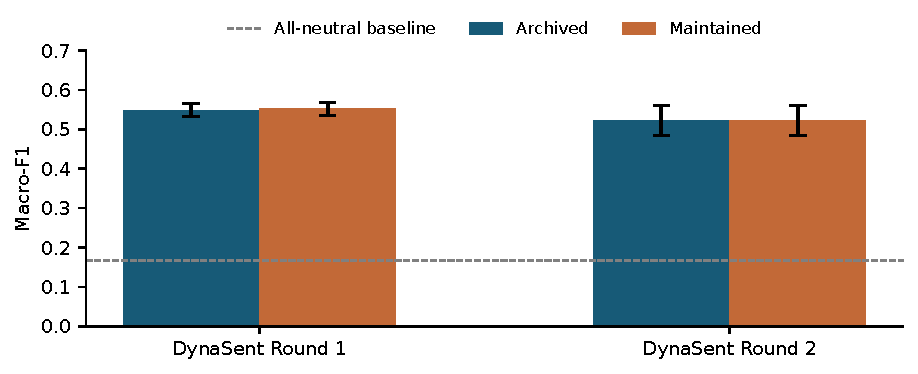
\includegraphics[width=.76\textwidth]{benchmark_f1.pdf}

\caption{MacroF1 with 95\% bootstrapped intervals. The two VADER implementations have similar performance on each official test split. The baseline hypothesis is that each item will be rated as neutral.}

\label{fig:user2}

\end{figure*}

In Round 1, the paired interval is $[-0.0022,0.0078]$ and in Round 2, the paired interval is $[-0.0079,0.0084]$. Both contain zero. The difference in implementation as observed on these sets is not large enough to support the claim of a credible improvement for maintained VADER when compared to sampling variation. The intervals are for uncertainty in the resampling of observed test data, and do not reflect uncertainty in all sampling methods.


Dror et al. (\hyperlink{ref_dror2018significance}{2018}) stress correlating statistical comparisons with task, metric and experimental design. Paired resampling maintains the same test examples for comparisons of implementations here.


More detail is provided with class-specific performance than with the headline score. The archived Round 2 negative recall is 0.408, while the positive items it is 0.617 (Table 6). Of 240 negative examples, 87 are predicted positive and 55 neutral. These figures indicate that context related negative evaluations are not yet easy to make. Additionally, the confusion is unlikely to be interpretable in a way that is just the model finding the correct sentiment but slightly mis-calibrating its intensity.


\begin{table}[t]
\centering\small
\setlength{\tabcolsep}{5pt}
\begin{tabular}{@{}lrrr@{}}
\toprule
Class & Precision & Recall & F1\\
\midrule
Negative & 0.544 & 0.408 & 0.467\\
Neutral & 0.554 & 0.554 & 0.554\\
Positive & 0.493 & 0.617 & 0.548\\
\bottomrule
\end{tabular}
\caption{Archived VADER on DynaSent Round 2. Each reference class has 240 items.}
\label{tab:user6}
\end{table}

\begin{figure*}[t]

\centering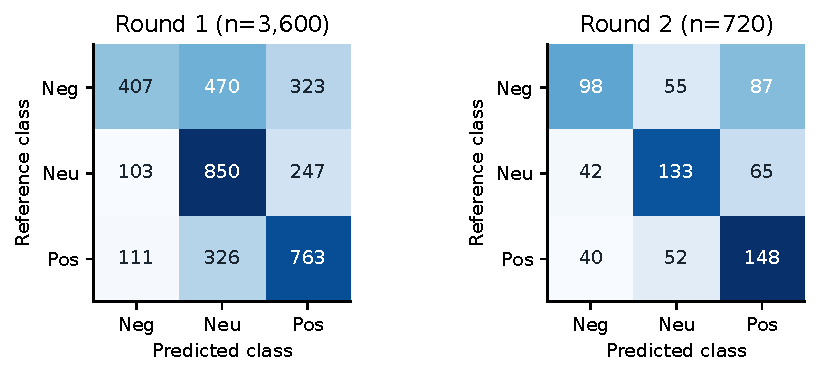
\includegraphics[width=.76\textwidth]{benchmark_confusion.pdf}

\caption{Archived VADER confusion matrices were generated. The rows contain human reference classes while the columns contain the predictions. There are a lot of negative items that appear the same in Round 1 but different in Round 2.}

\label{fig:user3}

\end{figure*}

Any conclusions about the classification results should be made within the context of the achieved classifications and not as a numerical comparison with the original Pearson correlations. But even comparison with the original provisional macro-F1 is to be exercised with caution since the original reference classes are based on intensity ratings, while DynaSent provides categorical labels. The change in score may result from a variety of domains, collection strategies and reference approaches. The experiments indicate there is a problem with transfers, though no one factor has been shown conclusively.


\subsection{Controlled behavioural diagnostics}

Table 7 shows the changes in scores for families that were not in the samples. The movement of positive-design families is toward the down incline of 0.704, while that of the negative-design families is toward the opposite slope of 0.688. Generally, modifier, capital and punctuation conditions add to the score in the base direction (not opposed to it. Contrast works to shift the mean towards the new opposing assessment introduced.


\begin{table*}[t]
\centering\small
\setlength{\tabcolsep}{5pt}
\begin{tabular}{@{}lrrrr@{}}
\toprule
Variant & Pos. \ensuremath{\Delta} & Check & Neg. \ensuremath{\Delta} & Check\\
\midrule
Negation & -0.704 & 10/12 & +0.688 & 11/12\\
Modifier & +0.041 & 10/12 & -0.052 & 11/12\\
Capitals & +0.095 & 10/12 & -0.122 & 11/12\\
Punctuation & +0.111 & 10/12 & -0.142 & 11/12\\
Contrast & -0.833 & 12/12 & +0.809 & 12/12\\
\bottomrule
\end{tabular}
\caption{Constructed diagnostics: ones with mean variant-minus-base compound change and with the count that satisfy the rules for the "drafting-direction" check. Tones are made into 12 families. Checks are not human measurements of accuracy, but are based on the design hypotheses created by AI. Base tones are either intended up or down---the positive or negative notation.}
\label{tab:user7}
\end{table*}

The direction-check count score is preliminary. Additionally, two positive design held-out bases are not reinforced by the variations of intensities, and one negative design family is also not reinforced. For example, the base for a dependable delivery crew is a zero archived compound score. In comparison, a straight-up closing-time sentence " cancels out" a factual help-desk sentence, which has the important value of 0.4019.In contrast, its negated form is not as clearly a negative telling of the service opinion as a factual help-desk closing-time sentence, whose score is 0.4019. The lexicon can be brought into operation on the context-free association of any word even if the whole sentence is a truthful statement.




The results, then, differentiate between success in the semantics and success in the execution of the rules. A sentiment token cannot be strengthened by a punctuation rule that the model doesn't recognize, and there can be a neutral description that pickles a sentiment induced by an active lexical entry. These cases can be inspected because of the 288 inputs and their predictions, but the excellent reference ratings are necessary to assign a human correctness score. These examples are not representative of the actual occurrence of each failure type in natural language as they have been picked out based on the scoring.


\subsection{LLM as judge pilot}

There are two within-session assistant judgements which comprise the evaluation. The DynaSent sample was created with 8240 as the seed number and selected to be 20 items from each released gold class. Ten families not used for development are included in the constructed sample, which includes all six variants. The only data included in the judge-input files are IDs and texts, no labels, no VADER scores and no condition names. The prompt requests one class, a supporting phrase, confidence and a brief explanation per item.


The judge in this conversation is the ChatGPT/ Codex assistant. No exact snapshot of the serving-model was available, no temperature and decoding seed was exposed. It wasn't some attempt running an external API. Input-preparing, output-recovering, prompts, and source limitations remain intact, and enables exact output-recovery of the recorded outputs. Closed models which yields the same results cannot be reproduced.


\begin{table}[t]
\centering\small
\setlength{\tabcolsep}{5pt}
\begin{tabularx}{\columnwidth}{@{}Xrr@{}}
\toprule
System on the same 60 items & Accuracy & Macro-F1\\
\midrule
Archived VADER & 0.500 & 0.498\\
Maintained VADER & 0.483 & 0.484\\
Assistant judge & 0.883 & 0.883\\
\bottomrule
\end{tabularx}
\caption{Exploratory comparison on the same balanced 60-item DynaSent sample. The assistant result is derived from preserved textual judgements that occur within the session.}
\label{tab:user8}
\end{table}

For the sample DynaSent items, the accuracy of the assistant is 0.883333 with macro-F1 score as 0.882784 and kappa with the released human class is 0.825. The macro-F1 accuracy of archived VADER with these items is 0.498074. The judge macro-F1 bootstrap interval is $[0.792,0.952]$. This is a useful contextual interpretation, but neither this small exploratory comparison nor any other comparison justifies making a broad statement about the assistant as a replacement for human annotation.


Mismatches between the inferred event valence and the overall sentiment label within the dataset are represented as the seven classes of imbued sentiment mismatches. The judge, for instance, discounts a threatening action as negative while releasing another item is neutral. A fragment has a neutral tag even if it was released with a positive tag. This becomes apparent in the differences, which shows the need for a plausible explanation to be no substitute for agreement with a declared reference policy.


VADER and the assistant difference in 44 of 60 labels (0.733333) on the built sample. This is only a model-to-model agreement. The assistant also wrote the created corpus and kept the overarching conversation context. The constructed trial is therefore not independently blinded and the included examples may be easier on the judge given that they are likely to be jointly written. Liu et al. (\hyperlink{ref_liu2023geval}{2023}) justify a structured model-based evaluation and note that there is evaluator bias, but do not confirm that this applies to a new adaptation of the sentiment classification task to generate evaluation experiments with good quality. Results are not yet available from comparison to real data human labels.


\section{Ethical considerations}

\subsection{Data, participation and attribution}

The Australian Code focuses on responsible conduct of research, reporting, responsible and honest use of research information, accurate acknowledgment \hyperlink{ref_researchCode}{(NHMRC et al., 2018)}. When applied to these or other aspects of software documentation, they suggest:ketae clear data provenance, preservation of unfavorable results, separation of evidence from plans and accurate code and annotations reuse attribution. If one fails or does not complete a replication, then it is reported as failed or incomplete instead of rectifying through the invisible mechanisms of changes.


Documenting the constructed corpus's motivation, composition, creation process and intended uses follows the transparency rationale of Gebru et al. (\hyperlink{ref_gebru2021datasheets}{2021}). All these properties along with the great human-validation limitation are described in its manifest and annotation guidelines.


Crowdsourced judgements were used in the original study. Their quality-control procedures and their collated references are a part of the published study, but this project does not represent a new consolation agreement or a re-examination of their original recruitment. The artefacts are released and the replication does not go so far as to re-identify owners of the adapted texts. Where copyright applies to the work, it is regarded as a source-access not a proprietary access.


An MIT notice is present on the upstream VADER code, and is retained. The repository and datasheet of DynaSent are discussed in this paper regarding Yelp's release \hyperlink{ref_dynasentData}{(Potts et al., 2026)} and possible inherited terms in Yelp. The public project will provide guidance on how to retrieve the contents of the source collections (or retrieval instructions and IDs and derived scores), not a replacement copy of the source collections. The source conditions are followed by a small evaluation sample in the local judge's records. The report or repository should not contain any API keys or credentials.


Proposed new annotation, with the involvement of volunteers. Authorised real participation should be based on course guidelines, always informed agreement, absence of unnecessary personal information in public documents and absence of participation unless a person chooses to stop. An anonymous reader codes is adequate for the computational audit. Records of consent and contacts should be kept confidential. No institution ethics approval or recruitment is claimed for this report.


\subsection{Model bias and interpretation}

VADER's lexicon and rules are language and rating conventions, in particular. An English short-text assessment may not be considered reliable in other languages, dialects, groups, or decisions in a specific area of specialization. The amount of the constructed corpus is limited in scope by the 4 service related domains and limited sentence forms. Stereotyped language and exemplified versions of the same language can be introduced with the assistance of AI. Any of the above negative, neutral and ambiguous cases requires independent annotation to test these assumptions and will minimize selective reporting.


Along with the sentiment output, it is necessary to operate it at the right level. A statement regarding a review sentence does not communicate the writer's psychological position, purpose, credibility or future actions. Such inferences are typically feeble given the amount of false positives in factual service descriptions. The present evaluation is for analysis for declared sentiment based tasks in text levels, that also supports individual profiling or implied decisions in consequence.


The other source of bias is the assistant judge. It may not be ruled out that it is trained with data drawn from a known public benchmark and there are no controls in the present user interface to enable the independent repeatability of a model trial. Where there is a conflict between its label and the reference, its explanations can be convincing even if the actual answers conflict. Record judgements of low confidence and keep human gold unchanged, minimises risk of treating fluency for correctness.


\subsection{Research integrity and AI assistance}

For the preparation of the soft copy, drafting of the corpus and preparation of a textual judge and report, generative AI proved helpful. Those values stored in the results are exported by the scripts executed during the report. Author Provenance and Judge Restriction disclosed. Human annotation was not simulated and no measurements were replaced to present as observations.


The student still bears the responsibility of reading and understanding the source papers, and the validation of the words submitted in accordance with the policy of the assessment: Open-AI. The planned work is not automatically described as completed, but is part of the unchanged files Assessment 1 and Assessment 2 which continue to be background evidence. As a result the novelty claim was changed to the DynaSent. These choices make final argument consistent with available experimental record.


\section{Conclusions and reflections}

Archived VADER can be successfully run with all published original texts and two of four correlations ran to three decimal places. Movie values and product values are not the same, and maintenance code has to be changed to improve the performance, but is not a solution for all discrepancies. The classification audit shows that results are significantly impacted by the classification via reference-score conversion and averaging over F1. Unfortunately, for one of the alternatives one has to accept, a tail-matching round-off headline is not enough to claim complete agreement with the original protocol.


Both implementations on the official DynaSent tests have similar macro-F1, with the value being approximately 0.55 around Round 1 and 0.52 around Round 2. Their errors are high relative to a constant class basis and they still have high class specific errors. This is because partial transfer occurs under fixed conditions. It does not mean that all modern short texts generally fail, nor is it an exhaustive list of sources of failure; it only states the domain shift is a source of failure.


The constructed corpus offers a transparent group of 288 similar inputs and shows correlations among lexical coverage and contextual rules. The within-session judge pilot provides supplement flexibility of interpretation, preserved outputs and explicit reproducible limits. An independent human annotation of the produced texts is still the predominant scientific need that is not completely met. The completion of it would allow for kappa (human-class reference measures) as well as intensity correlation and paired family-level analysis, thereby answering the third research question in the desired way.


What conclusions may be drawn from the numbers is determined by the data identity, reference policy, and human or model judgement for the selection of versions. Decisions made with these scripts are included with the script and are auditable.


\clearpage
\begin{thebibliography}{}

\bibitem[COMP8240(2026)]{courseCriteria2026} \hypertarget{ref_courseCriteria2026}{}2026. COMP8240 overall goal and assessment criteria. Unit iLearn guidance, Session 2.

\bibitem[Ron Artstein and Massimo Poesio(2008)]{student-ref-211} \hypertarget{ref_artstein2008agreement}{} Ron Artstein and Massimo Poesio. 2008. \href{https://doi.org/10.1162/coli.07-034-R2}{Survey article: Inter-coder agreement for computational linguistics}. \emph{Computational Linguistics}, 34(4):555--596.

\bibitem[Jacob Cohen(1960)]{student-ref-212} \hypertarget{ref_cohen1960agreement}{}Jacob Cohen. 1960. \href{https://doi.org/10.1177/001316446002000104}{A coefficient of agreement for nominal scales}. \emph{Educational and Psychological Measurement}, 20(1):37--46.

\bibitem[Computing Research and Education Association of Australasia(2023)]{student-ref-213} \hypertarget{ref_core2023}{}Computing Research and Education Association of Australasia. 2023. \href{https://portal.core.edu.au/conf-ranks/?search=ICWSM\&by=all\&source=CORE2023}{CORE2023 conference rankings: ICWSM}. Historical ranking, accessed 4 November 2026.

\bibitem[Rotem Dror, Gili Baumer, Segev Shlomov, and Roi Reichart(2018)]{student-ref-214} \hypertarget{ref_dror2018significance}{}Rotem Dror, Gili Baumer, Segev Shlomov, and Roi Reichart. 2018. \href{https://doi.org/10.18653/v1/P18-1128}{The hitchhiker's guide to testing statistical significance in natural language processing}. In \emph{Proceedings of the 56th annual meeting of the association for computational linguistics (volume 1: Long papers)}, pages 1383--1392. Association for Computational Linguistics.

\bibitem[Timnit Gebru, Jamie Morgenstern, Briana Vecchione, Jennifer Wortman Vaughan, Hanna Wallach, Hal Daumé III, and Kate Crawford(2021)]{student-ref-215} \hypertarget{ref_gebru2021datasheets}{}Timnit Gebru, Jamie Morgenstern, Briana Vecchione, Jennifer Wortman Vaughan, Hanna Wallach, Hal Daumé III, and Kate Crawford. 2021. \href{https://doi.org/10.1145/3458723}{Datasheets for datasets}. \emph{Communications of the ACM}, 64(12):86--92.

\bibitem[C. J. Hutto(2026)]{student-ref-216} \hypertarget{ref_huttoCode}{}C. J. Hutto. 2026. \href{https://github.com/cjhutto/vaderSentiment/tree/44fc044cd877310ee8278a0eadf34bcd50d41d06}{VADER sentiment analysis: Author code and original study resources}. Pinned revision 44fc044c; accessed 4 November 2026.

\bibitem[C. J. Hutto and Eric Gilbert(2014)]{student-ref-217} \hypertarget{ref_hutto2014vader}{}C. J. Hutto and Eric Gilbert. 2014. \href{https://doi.org/10.1609/icwsm.v8i1.14550}{VADER: A parsimonious rule-based model for sentiment analysis of social media text}. In \emph{Proceedings of the international AAAI conference on web and social media}, volume 8, pages 216--225.

\bibitem[Yang Liu, Dan Iter, Yichong Xu, Shuohang Wang, Ruochen Xu, and Chenguang Zhu(2023)]{student-ref-218} \hypertarget{ref_liu2023geval}{}Yang Liu, Dan Iter, Yichong Xu, Shuohang Wang, Ruochen Xu, and Chenguang Zhu. 2023. \href{https://doi.org/10.18653/v1/2023.emnlp-main.153}{G-Eval: NLG evaluation using GPT-4 with better human alignment}. In \emph{Proceedings of the 2023 conference on empirical methods in natural language processing}, pages 2511--2522. Association for Computational Linguistics.

\bibitem[NHMRC, Australian Research Council, and Universities Australia(2018)]{student-ref-219} \hypertarget{ref_researchCode}{}NHMRC, Australian Research Council, and Universities Australia. 2018. \href{https://www.nhmrc.gov.au/about-us/publications/australian-code-responsible-conduct-research-2018}{Australian code for the responsible conduct of research}.

\bibitem[Bo Pang and Lillian Lee(2008)]{student-ref-220} \hypertarget{ref_pang2008opinion}{}Bo Pang and Lillian Lee. 2008. \href{https://www.cs.cornell.edu/home/llee/opinion-mining-sentiment-analysis-survey.html}{Opinion mining and sentiment analysis}. \emph{Foundations and Trends in Information Retrieval}, 2(1--2):1--135.

\bibitem[Joelle Pineau, Philippe Vincent-Lamarre, Koustuv Sinha, Vincent Lariviere, Alina Beygelzimer, Florence d'Alché-Buc, Emily Fox, and Hugo Larochelle(2021)]{student-ref-221} \hypertarget{ref_pineau2021reproducibility}{}Joelle Pineau, Philippe Vincent-Lamarre, Koustuv Sinha, Vincent Lariviere, Alina Beygelzimer, Florence d'Alché-Buc, Emily Fox, and Hugo Larochelle. 2021. \href{https://www.jmlr.org/papers/v22/20-303.html}{Improving reproducibility in machine learning research (a report from the NeurIPS 2019 reproducibility program)}. \emph{Journal of Machine Learning Research}, 22(164):1--20.

\bibitem[Christopher Potts, Zhengxuan Wu, Atticus Geiger, and Douwe Kiela(2021)]{student-ref-222} \hypertarget{ref_potts2021dynasent}{}Christopher Potts, Zhengxuan Wu, Atticus Geiger, and Douwe Kiela. 2021. \href{https://doi.org/10.18653/v1/2021.acl-long.186}{DynaSent: A dynamic benchmark for sentiment analysis}. In \emph{Proceedings of the 59th annual meeting of the association for computational linguistics and the 11th international joint conference on natural }\emph{language processing (volume 1: Long papers)}, pages 2388--2404. Association for Computational Linguistics.

\bibitem[Christopher Potts, Zhengxuan Wu, Atticus Geiger, and Douwe Kiela(2026)]{student-ref-223} \hypertarget{ref_dynasentData}{}Christopher Potts, Zhengxuan Wu, Atticus Geiger, and Douwe Kiela. 2026. \href{https://github.com/cgpotts/dynasent/tree/707b6208978bfe7ff251a0c3263c9f0552c27b48}{DynaSent version 1.1: Data release and datasheet}. Pinned revision 707b6208; accessed 4 November 2026.

\bibitem[Marco Tulio Ribeiro, Tongshuang Wu, Carlos Guestrin, and Sameer Singh(2020)]{student-ref-224} \hypertarget{ref_ribeiro2020checklist}{}Marco Tulio Ribeiro, Tongshuang Wu, Carlos Guestrin, and Sameer Singh. 2020. \href{https://doi.org/10.18653/v1/2020.acl-main.442}{Beyond accuracy: Behavioral testing of NLP models with CheckList}. In \emph{Proceedings of the 58th annual meeting of the association for computational linguistics}, pages 4902--4912. Association for Computational Linguistics.

\bibitem[scikit-learn developers(2026)]{student-ref-225} \hypertarget{ref_sklearnMetrics}{}scikit-learn developers. 2026. \href{https://sklearn.org/stable/modules/generated/sklearn.metrics.f1_score.html}{F1 score: Metric definition and averaging options}. Accessed 4 November 2026; experiments use scikit-learn 1.8.0.

\bibitem[Jiaxu Wang, Bowen Rong, Chengcheng Li, Huiying Xu, and Xinzhong Zhu(2026)]{student-ref-226} \hypertarget{ref_wang2026msra}{}Jiaxu Wang, Bowen Rong, Chengcheng Li, Huiying Xu, and Xinzhong Zhu. 2026. \href{https://doi.org/10.3390/electronics15184230}{MSRA-CCL: Multi-source reliability-aware aggregation and cross-domain consistency learning for weakly supervised sentiment classification}. \emph{Electronics}, 15(18):4230.

\bibitem[Theresa Wilson, Janyce Wiebe, and Paul Hoffmann(2005)]{student-ref-227} \hypertarget{ref_wilson2005contextual}{}Theresa Wilson, Janyce Wiebe, and Paul Hoffmann. 2005. \href{https://aclanthology.org/H05-1044/}{Recognizing contextual polarity in phrase-level sentiment analysis}. In \emph{Proceedings of human language technology conference and conference on empirical methods in natural language processing}, pages 347--354. Association for Computational Linguistics.

\end{thebibliography}

\clearpage
\onecolumn
\appendix
\section{Supplementary figure}
\begin{figure}[!ht]

\centering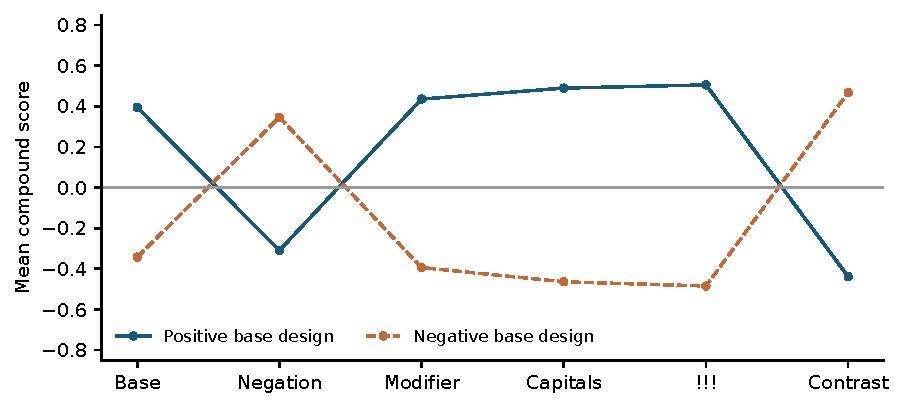
\includegraphics[width=.88\textwidth]{constructed_scores.pdf}

\caption{Means of compound scores in the 24 held out families who were drafted with positive and negative base tones were archived. In this plot, the mean scores for maintained students and those that are not maintained are the same. Lines indicate the behaviour of the numerical model. They do not constitute an agreement with the independent human interpretation.}

\label{fig:user4}

\end{figure}
\end{document}
